\documentclass[11pt,t]{beamer}
%% Language and font encodings
\usepackage[english]{babel}
\usepackage[utf8x]{inputenc}
\usepackage[T1]{fontenc}

\usepackage{helvet}

%% Sets page size and margins
\usepackage[letterpaper,top=3cm,bottom=2cm,left=3cm,right=3cm,marginparwidth=1.75cm]{geometry}

%% Useful packages
\usepackage{amsmath}
\usepackage{graphicx}
\usepackage{tcolorbox}
\usepackage{amssymb}
\usepackage{amsthm}
\usepackage{lastpage}
\usepackage{accents}
\usepackage{multicol}

% For better list numbering
\usepackage[shortlabels]{enumitem}

% Font
% \usepackage{tgbonum}


% Tikz
\usepackage{tikz}

\usetikzlibrary{calc,fit,shapes.misc,backgrounds}
\usepackage{pgfplots}
\pgfplotsset{compat = newest}
\usetikzlibrary{positioning, arrows.meta}
\usepgfplotslibrary{fillbetween}

% Headers
\usepackage{fancyhdr}
\pagestyle{fancy}

% Store \@title as \thetitle
\makeatletter
\let\thetitle\@title
\makeatother

\fancyhf{}
\lhead{\fontfamily{qbk}\fontsize{10}{11}\selectfont ECON 3070}
\rhead{\fontfamily{qbk}\fontsize{10}{11}\selectfont \thetitle}
\rfoot{\fontfamily{qbk}\fontsize{10}{11}\selectfont \thepage}


% Sections and Subsections

% define colors
\definecolor{buff-gold}{HTML}{CFB87C}
\definecolor{buff-grey}{HTML}{565A5C}
% custom tcolorbox
\tcbset{colframe=buff-gold, colback=white!100!black}

% new page per section
\usepackage{titlesec}
\newcommand{\sectionbreak}{\clearpage}
% change style of section
\usepackage{sectsty}
\sectionfont{\color{buff-gold} \fontfamily{qbk}\selectfont}
\subsectionfont{\color{buff-grey} \fontfamily{qbk}\selectfont}


\author{Kyle Butts}
\title{Lecture 10 - Competitive Markets: Applications}
\subtitle{ECON 3070 - Intermediate Microeconomic Theory}

\begin{document}

\begin{frame}
  \titlepage
\end{frame}

\begin{frame}{Overview}
  In the previous chapter, we defined a perfectly competitive market, and learned how to calculate short-run and long-run equilibria

  \begin{itemize}
    \item We discussed the long-run equilibrium outcome (zero profit)
  \end{itemize}

  In this chapter, we will look at the impact of government interventions in perfectly competitive markets

  \begin{itemize}
    \item These include taxes and subsidies, prices floors and ceilings, and production quotas
  \end{itemize}
\end{frame}

\begin{frame}{Introduction}
  In this chapter, we will be considering the impacts of government interventions in a specific market.

  \begin{itemize}
    \item However, we will ignore spillover effects of these interventions into other markets
  \end{itemize}

  \bigskip
  That is, we will be considering the partial equilibrium effects, as opposed to the general equilibrium effects

  \begin{itemize}
    \item A \textbf{partial equilibrium} approach focuses only on a single market (for example, the housing market).
    \item A \textbf{general equilibrium} approach considers how changes in that market might affect other markets.
  \end{itemize}  

\end{frame}

\begin{frame}{Introduction}
  We will also be ignoring any potential externalities.

  \bigskip
  An \textbf{externality} is a cost or benefit borne on a third party, which is not reflected in the price of the product in that market.
  
  \begin{itemize}
    \item For example, pollution from cars, or herd effects of vaccination.
  \end{itemize}
\end{frame}

\begin{frame}{The Invisible Hand}
  Why is a competitive market economically efficient (surplus maximizing)?

  \bigskip
  \textbf{When the demand curve is above the supply curve, there is a consumer who is willing to pay more for the good than it costs to produce.}

  \begin{itemize}
    \item If additional units are sold, consumer and/or producer surplus will increase.
  \end{itemize}
\end{frame}

\begin{frame}{The Invisible Hand}
  \textbf{But if the demand curve is below the supply curve, additional consumers receive less benefit from the good than it costs to produce.}

  \begin{itemize}
    \item If additional units are sold, consumer and/or producer surplus will decrease.
  \end{itemize}

  \pause\bigskip
  In a competitive market, there is no central planner arranging transactions.

  \begin{itemize}
    \item Yet decentralized decision-making by individual consumers and producers maximizes total surplus...
    
    \item As if the economy is guided by an \textit{invisible hand}.
  \end{itemize}  
\end{frame}

\begin{frame}{The Invisible Hand}

  \begin{columns}[T]
    \vspace{0pt}
    \begin{column}{.55\textwidth}
      \begin{figure}
        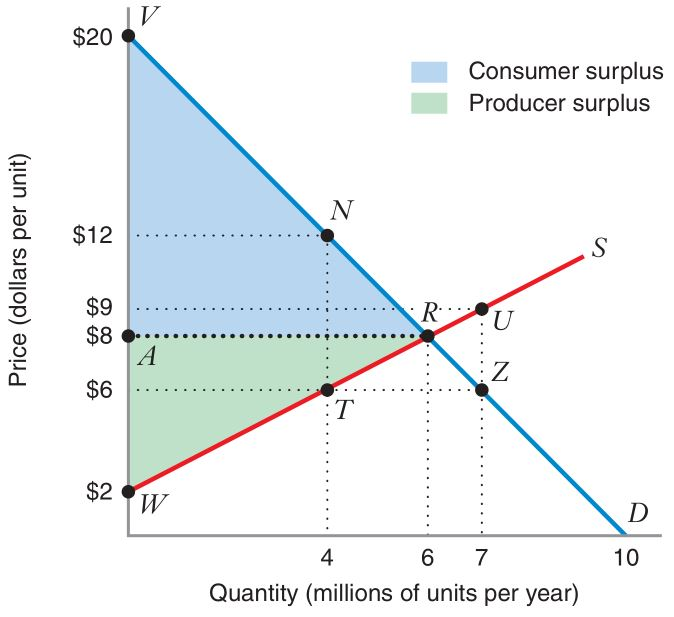
\includegraphics[width=\textwidth]{figures/fig10_1.jpg}
      \end{figure}

      \vspace*{50mm} % Ensures columns are up top; delete if you want columns centered on page
    \end{column}
    
    \hfill
    
    \begin{column}{.45\textwidth}
      {\color{accent}\rule{\linewidth}{2pt}}

      \begin{itemize}
        \item Notice that all trades where Willingness to Pay $ > $ Marginal Cost occur
        \item And no sale where WTP $ < $ MC occurs
        \item Thus, the market is maximizing total surplus
      \end{itemize}
    \end{column}
  \end{columns}

\end{frame}


\begin{frame}{Excise Taxes}
  An \textbf{excise tax} is a tax on a specific commodity, such as gasoline, tobacco, or tea.

  \begin{itemize}
    \item In the absence of a tax, the price paid for the good by the consumer will equal the price received by the producer.
    
    \item That is, $Q_d(P)=Q_s(P)$.
  \end{itemize}

  \bigskip \pause
  However, when a tax is imposed, it creates a ``tax wedge" between the price paid and the price received.

  For example, if the government imposes a \$6 tax on gasoline, then
  $$
    P_s=P_d-6 \text{ or } P_s+6=P_d
  $$
\end{frame}

\begin{frame}{Excise Tax}
  \begin{columns}[T]
    \vspace{0pt}
    \begin{column}{.55\textwidth}
      \begin{figure}
        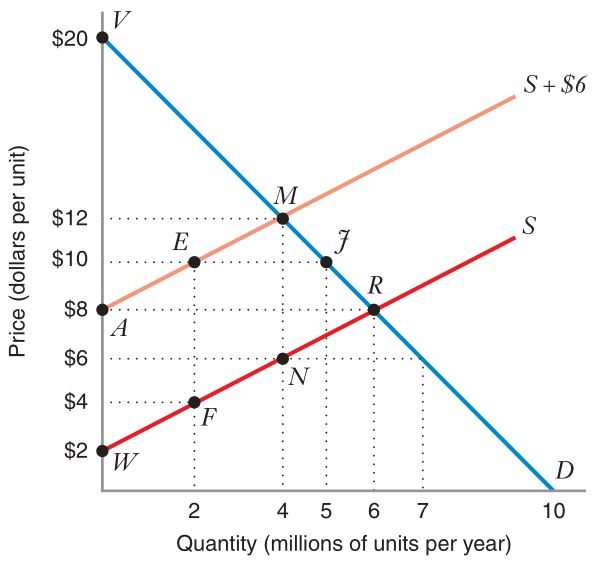
\includegraphics[width=\textwidth]{figures/fig10_2.jpg}
      \end{figure}

      \vspace*{50mm} % Ensures columns are up top; delete if you want columns centered on page
    \end{column}
    
    \hfill
    
    \begin{column}{.45\textwidth}
      {\color{accent}\rule{\linewidth}{2pt}}

      \begin{itemize}
        \item The shifted supply curve intersects demand at $M$ with $Q = 4$ and a price of $P_d = \$12$. 
        \item However, the seller only receives $P_s = \$6$ at the point $N$ because of the tax
      \end{itemize}
    \end{column}
  \end{columns}
\end{frame}

\begin{frame}{Excise Taxes}
  In this case, the market will underproduce relative to the efficient level.

  \begin{itemize}
    \item Consumer surplus will be lower from a higher $P_d$
    \item Producer surplus will be lower from a lower $P_s$
    \item The government will receive some revenue from the tax, $\$6$ per unit 
  \end{itemize}
  
  \bigskip
  Overall, the total surplus before the tax will be larger than the total surplus + tax revenue after the tax
  
  \begin{itemize}
    \item A \textbf{deadweight loss} (in total surplus) will be created
  \end{itemize}
\end{frame}

\begin{frame}{Excise Tax}
  The deadweight loss is a result of the fact that the amount of gov't revenue gained through the taxis less than the consumer and producer surplus lost as a result of the tax.

  \bigskip\pause
  Economically, the deadweight loss from an excise tax is a result of forgone market transactions where the marginal benefit gained to the consumer would exceed the marginal cost to the producer.
\end{frame}

\begin{frame}{Excise Tax}
  \begin{columns}[T]
    \vspace{0pt}
    \begin{column}{.6\textwidth}
      \begin{figure}
        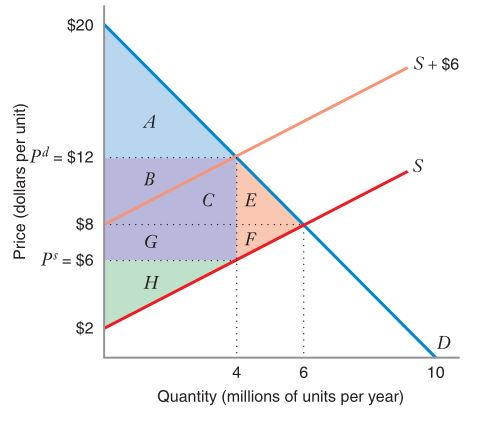
\includegraphics[width=\textwidth]{figures/fig10_3a.jpg}
      \end{figure}

      \vspace*{50mm} % Ensures columns are up top; delete if you want columns centered on page
    \end{column}
    
    \hfill
    
    \begin{column}{.4\textwidth}
      {\color{accent}\rule{\linewidth}{2pt}}

      \textbf{Before:} 
      
      Total Surplus $= A + B + C + E + F + G + H$
      
      \bigskip
      \textbf{After:}

      Consumer Surplus $= A$
      
      Producer Surplus $= H$
      
      Tax Revenue $= B + C + G$
      
      \bigskip
      \textbf{Loss in Surplus:}

      Deadweight Loss $= E + F$
    \end{column}
  \end{columns}
\end{frame}

\begin{frame}{Excise Tax}
  Let's look at an example of the impact of an excise tax on the equilibrium quantity and price in a perfectly competitive market. Suppose $Q_d = 10 - 0.5 P_d$ and $Q_s = P_s - 2$.

  \bigskip
  Without the tax, the market equilibrium is where $Q_s = Q_d$, and $P_s = P_d$.

  \pause
  $$
    10 - 0.5P = P - 2 \Rightarrow 12 = 1.5P \Rightarrow P^* = 8
  $$

  At the price $P^* = 8$, we have $Q_s(8) = Q_d(8) = 6$ units.
\end{frame}

\begin{frame}{\bgCoral{Try It Yourself}}
  From the previous example, what is the producer surplus in the market, absent the tax?
\end{frame}

\begin{frame}{Excise Tax}
  Now suppose that the gov't imposes a tax of \$6. The market equilibrium is still where $Q_s = Q_d$, but $P_s = P_d - 6$
  
  \pause
  $$
  10 - 0.5P_d = (P_d - 6) - 2  \Rightarrow 18 = 1.5P_d \Rightarrow P_d^* = 12 
  $$

  \pause\medskip
  That is the price buyers pay. To calculate the price sellers receive, $P_s^* = P_d^* - 6 = 12 - 6 = 6$. Finally, $Q_d = Q_s = P_s - 2 = 4$ units.
\end{frame}

\begin{frame}{\bgCoral{Try It Yourself}}
  From the previous example, what is the \textbf{change in} producer surplus resulting from the tax?
\end{frame}

\begin{frame}{Excise Tax}
  Note that with the imposition of the tax, 2 fewer units were sold.

  \begin{itemize}
    \item This means that there were two consumers whose WTP exceeded the marginal cost...
    \item ...that were no longer willing to buy the good after the tax.
  \end{itemize}

  \bigskip
  The deadweight loss is due to these forgone transactions.
\end{frame}

\begin{frame}{Incidence of a Tax}
  Note that in the previous example, we didn't pay attention to who was paying the tax. It turns out, it doesn't matter who you tax, the result is the same!
  
  \pause\bigskip
  And although the tax was \$6, 
  \begin{itemize}
    \item The price paid by consumers only increased by \$4
    \item The price received by sellers fell by \$2
  \end{itemize}

  In some sense, the consumers paid more of the tax than the sellers.

  \pause \bigskip
  The \textbf{incidence of the tax} refers to the effect that the tax has on the prices that consumers pay and that sellers receive.
\end{frame}

\begin{frame}{Incidence of a Tax}
  \emph{Who has the larger incidence in each example?}
  \begin{figure}
    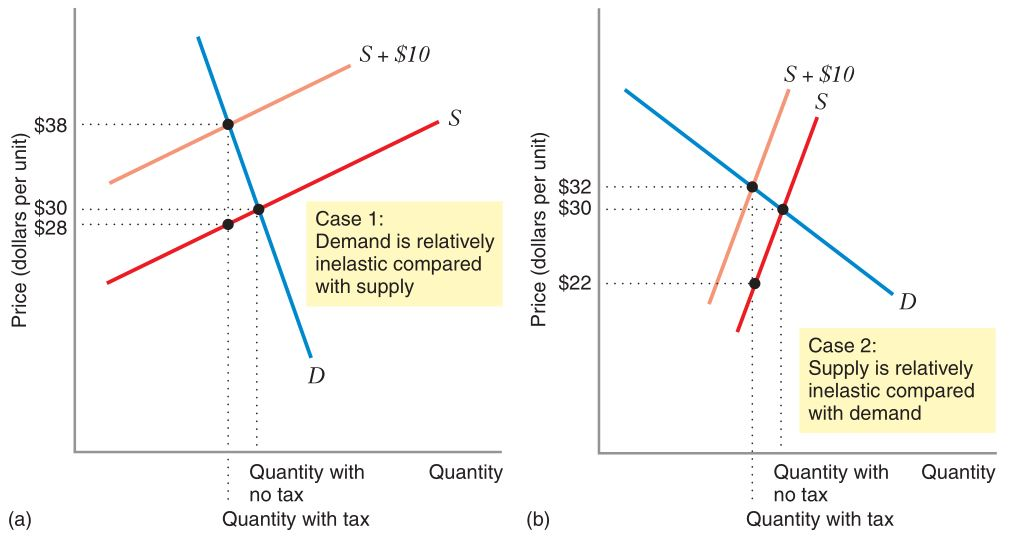
\includegraphics[width=300px]{figures/fig10_4.jpg}
  \end{figure}
\end{frame}

\begin{frame}{Incidence of a Tax}
  If demand is relatively \textit{inelastic} compared to supply, then consumers are less sensitive to a price change

  \begin{itemize}
    \item the consumers will bear more of the burden of the tax
  \end{itemize}

  \bigskip
  On the other hand, if demand is relatively \textit{elastic} compared to supply
  \begin{itemize}
    \item the producers will bear more of the burden
  \end{itemize}

  \bigskip
  The incidence of a tax does not depend on who the tax is levied on!
\end{frame}



\begin{frame}{\bgCoral{Try It Yourself}}

  Suppose that demand for sugary beverages is \textbf{perfectly inelastic}, and that supply is \textbf{relatively elastic}. What will the effect be of a \$3 tax on the price paid by consumers ($P_d$), and the price received by sellers ($P_s$)? \emph{(Hint: Draw the supply and demand curves)}

  \bigskip
  \begin{enumerate}[A)]
    \item $P_d$ will increase by \$3, and $P_s$ will not change
    \item $P_d$ will not change, and $P_s$ will decrease by \$3
    \item $P_d$ will increase by \$1.50, and $P_s$ decrease by \$1.50
    \item $P_d$ will not change, and $P_s$ will increase by \$3
  \end{enumerate}
\end{frame}

\begin{frame}{Subsidies}
  A subsidy can be thought of as a negative tax.
  \begin{itemize}
    \item When a subsidy of \$T is offered by the government, the effect is basically the opposite of a tax.
  \end{itemize}

  \bigskip\pause
  The new market equilibrium will be such that $P_s = P_d + \$T$

  \begin{itemize}
    \item The market will overproduce the good.
    \item Consumer surplus will be higher.
    \item Producer surplus will be higher.
    \item The government must spend money on the subsidy.
    \item A deadweight loss will be created.
  \end{itemize}
\end{frame}


\begin{frame}{Subsidies}
  \begin{columns}[T]
    \vspace{0pt}
    \begin{column}{.55\textwidth}
      \begin{figure}
        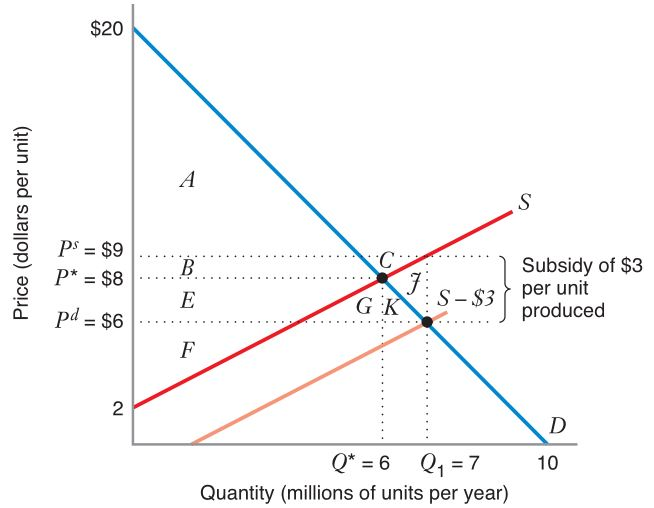
\includegraphics[width=\textwidth]{figures/fig10_6a.jpg}
      \end{figure}

      \vspace*{50mm} % Ensures columns are up top; delete if you want columns centered on page
    \end{column}
    
    \hfill
    
    \begin{column}{.45\textwidth}
      {\color{accent}\rule{\linewidth}{2pt}}

      \begin{itemize}
        \item The subsidies increases quantity to $Q_1 = 7$
        
        \item Consumers pay \$2 less and producers receive \$1 more, so they're both happy
        
        \item The government pays \$3 per unit which outweights the increase in surplus
      \end{itemize}
    \end{column}
  \end{columns}
\end{frame}

\begin{frame}{Subsidies}
  In this case, the deadweight loss is a result of the fact that gov't expenditures on the subsidy exceed the increase in total surplus

  \bigskip
  Economically, some consumers are encouraged to buy when the marginal cost to producers actually exceeds their marginal benefit, leading to negative total surplus.
\end{frame}

\begin{frame}{Price Ceilings}
  A \textbf{price ceiling} mandates that the price of a commodity cannot rise above a given level (e.g. rent controls).

  \begin{itemize}
    \item In order to be binding, the price ceiling must be below the market price.
  \end{itemize}

  \bigskip
  In this case, the lower price results in lower quantity supplied, and higher quantity demanded

  \begin{itemize}
    \item And thus, a shortage is created (excess demand)
  \end{itemize}
\end{frame}

\begin{frame}{Price Ceilings}
  As a result of a price ceiling, producer surplus will be lower because the 
  \begin{itemize}
    \item the market price is lower 
    \item textbf{and} some producers will exit the market
  \end{itemize}

  \bigskip
  Some of that producer surplus will be transferred to consumer surplus (due to the lower price).

  \begin{itemize}
    \item However, some consumer surplus may be lost due to the lack of available supply (magnitude depends on who gets the existing supply).
  \end{itemize}

  \bigskip
  Finally, there will be deadweight loss due to foregone transactions.
\end{frame}

\begin{frame}{Price Ceilings}
  50 units are sold, but you don't know which consumers can buy it, hence consumer surplus is ambiguous
  \begin{figure}
    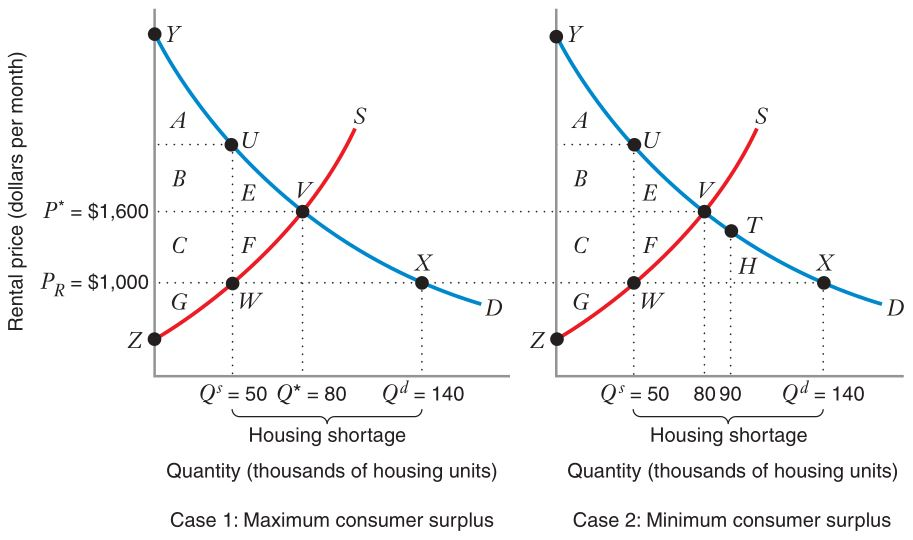
\includegraphics[width=0.8\textwidth]{figures/fig10_7a.jpg}
  \end{figure}
\end{frame}

\begin{frame}{Food Shortages in Venezuela}
  \begin{columns}[T]
    \vspace{0pt}
    \begin{column}{.55\textwidth}
      \begin{figure}
        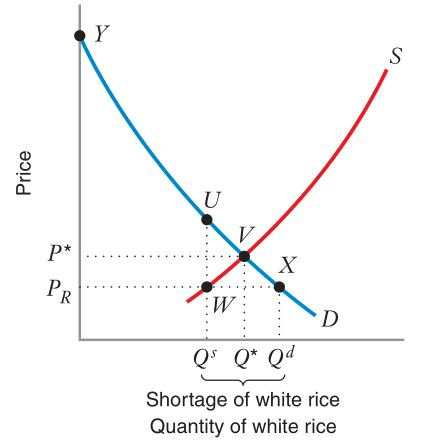
\includegraphics[width=\textwidth]{figures/fig10_8.jpg}
      \end{figure}

      \vspace*{50mm} % Ensures columns are up top; delete if you want columns centered on page
    \end{column}
    
    \hfill
    
    \begin{column}{.45\textwidth}
      {\color{accent}\rule{\linewidth}{2pt}}

      In 2003, Venezuela's president imposed price ceilings on many household goods as a result of inflation.

      \begin{itemize}
        \item By 2009, 400 food items had mandated price ceilings.
        
        \item Today, Venezuela is still plagued by food shortages as a result.
      \end{itemize}
    \end{column}
  \end{columns}
\end{frame}

\begin{frame}{Price Floors}
  A \textbf{price floor} mandates that the price of a commodity cannot fall below a given level.
  
  \begin{itemize}
    \item An example is a minimum wage.
    
    \item A price floor must be above the market price in order to be binding.
  \end{itemize}

  \bigskip The result of a price floor is that quantity demanded falls, and quantity supplied rises.

  \begin{itemize}
    \item Yielding a surplus of the commodity (excess supply).
  \end{itemize}
\end{frame}


\begin{frame}{Price Floors}
  A price floor will lower consumer surplus:

  \begin{itemize}
    \item Some consumers will be forced out of the market
    \item \textbf{and} others will be paying a higher price than before.
  \end{itemize}
  
  \bigskip
  Some of that will become producer surplus, as those producers are paid more.

  \bigskip
  But for those customers who are pushed out of the market, their consumer surplus disappears creating deadweight loss
\end{frame}

\begin{frame}{Price Floors}
  \begin{columns}[T]
    \vspace{0pt}
    \begin{column}{.55\textwidth}
      \begin{figure}
        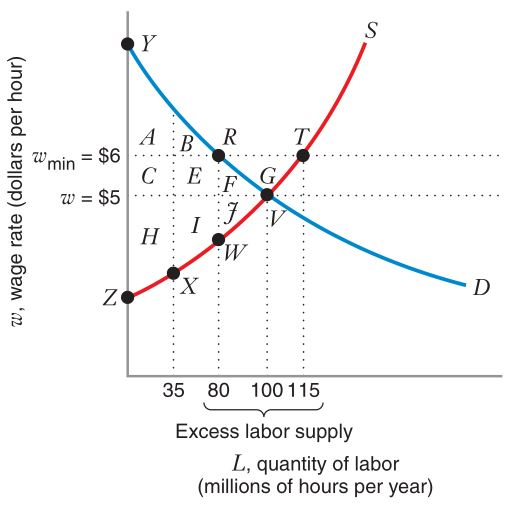
\includegraphics[width=\textwidth]{figures/fig10_10a.jpg}
      \end{figure}

      \vspace*{50mm} % Ensures columns are up top; delete if you want columns centered on page
    \end{column}
    
    \hfill
    
    \begin{column}{.45\textwidth}
      {\color{accent}\rule{\linewidth}{2pt}}

      \begin{itemize}
        \item At the minimum wage of \$6, 115 units of labor will be supplied but only 80 units will be demanded (excess supply)
        
        \item Therefore, only \$80 units will be bought at a price of \$6

        \item The deadweight loss $= F + J$
      \end{itemize}
    \end{column}
  \end{columns}
\end{frame}

\begin{frame}{\bgCoral{Try It Yourself}}
  Which of the following statements is false?

  \bigskip
  \begin{enumerate}[A)]
    \item With a price floor, the market will not clear.
    \item With a price floor, consumers will buy less of the good than they would in a free market.
    \item With a price floor, producer surplus will always increase.
    \item With a price floor there will be excess supply.
  \end{enumerate}
\end{frame}

\begin{frame}{Conclusion}
  In the previous few chapters, we defined a perfectly competitive market, and analyzed the implications of our assumptions.

  \begin{itemize}
    \item We also looked at a few applications of perfectly competitive markets
  \end{itemize}

  \medskip
  In the next few chapters, we will relax some of those assumptions, and look at markets that are not perfectly competitive.

  \begin{itemize}
    \item For example, monopolies and oligopolies.
  \end{itemize}
  
  \medskip
  Time permitting, we will also consider scenarios where perfectly competitive markets fail to maximize social welfare (total surplus) due to externalities.
\end{frame}
\end{document}
